\documentclass[fullscreen=true, bookmarks=true, hyperref={pdfencoding=unicode}]{beamer}
\usepackage[utf8]{inputenc}                                % Кодировка
\usepackage[english,russian]{babel}                        % Переносы
\usepackage{xcolor}                                        % Работа с цветом
\usepackage{amsmath,amssymb,amsfonts}                      % Символы АМО
\usepackage{graphicx}                                      % Графика
\usepackage[labelsep=period]{caption}                      % Разделитель в подписях к рисункам и таблицам
\usepackage{hhline}                                        % Для верстки линий в таблицах
\usepackage{tikz}                                          % Для простых рисунков в документе
\usepackage{fancybox}                                      % Пакет для отрисовки рамок
\usepackage{verbatim}                                      % Для вставки кода в презентацию
\usepackage{animate}                                       % Для вставки видео в презентацию
\usepackage{xmpmulti}                                      % Для вставки gif в презентацию
\usepackage{multirow}

\usetikzlibrary{arrows,snakes,backgrounds}                 % Для отрисовки стрелок

\graphicspath{{images/}}                                   % Путь до рисунков
\setbeamertemplate{caption}[numbered]                      % Включение нумерации рисунков

\definecolor{links}{HTML}{2A1B81}                          % blue for url links
\hypersetup{colorlinks,linkcolor=,urlcolor=links}          % nothing for others

\usetheme{boxes}
\usecolortheme{crane}

\newtheorem*{question}{Вопрос}

\title{Лекция 7. Гауссовские процессы}
\author{Петр Мостовский}
\institute{МКН СПбГУ}
\date{31 марта 2022}
\titlegraphic{
\includegraphics[keepaspectratio,width=0.5\textwidth]{logo_fmkn.png}}

\begin{document}
%\unitlength=2mm

% выводим заглавие
\begin{frame}
    \transdissolve[duration=0.2]
    \titlepage
\end{frame}


\begin{frame}
  \frametitle{Пятиминутка}
  \begin{itemize}
    \item Выпишите разложение параметров тематической модели через матрицы вероятностей терминов в теме и тем в документе
    \item Опишите, что такое распределение Дирихле (Latent Dirichlet Allocation, LDA), можно без формул
    \item Приведите ключевые идеи модели word2vec
  \end{itemize}
\end{frame}


\begin{frame}{}

    \centerline{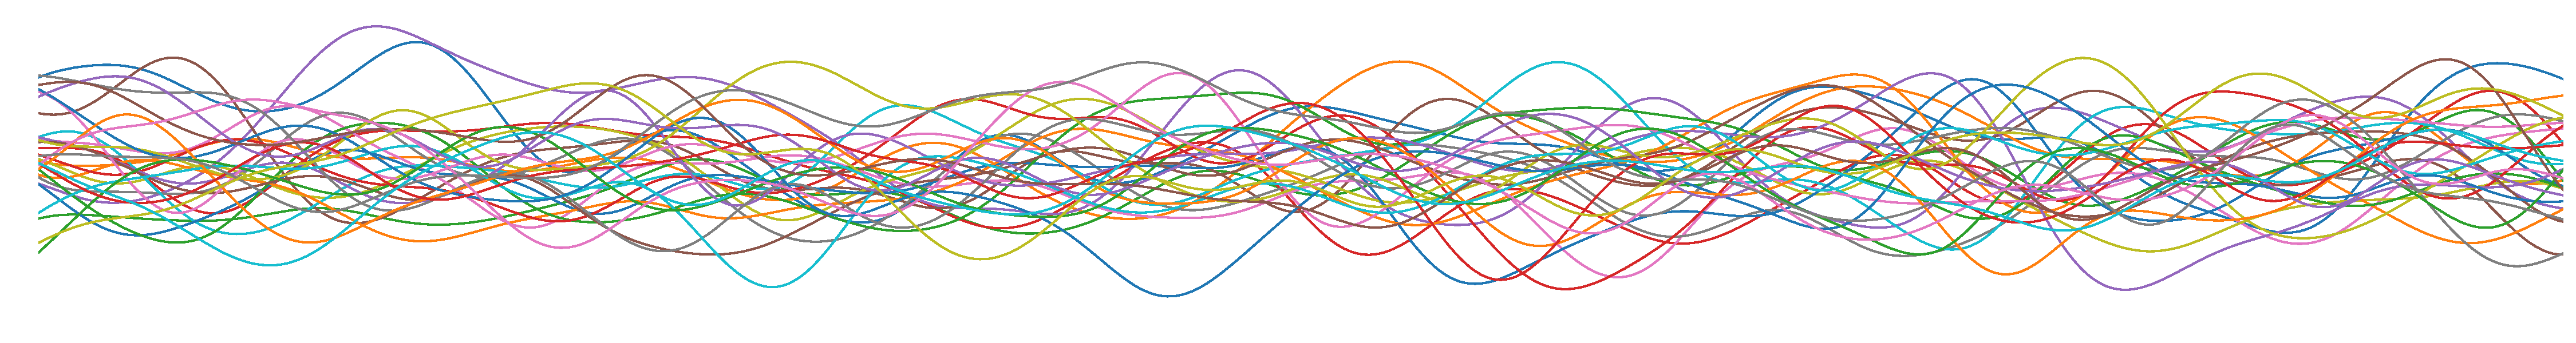
\includegraphics[]{logo-samples.pdf}}

\end{frame}


\begin{frame}{Напоминание о теореме Байеса}

    $$ P(A | B) = \frac{P(B | A) P(A)}{\int P(B | A) P(A) dA} = \frac{P(B | A) P(A)}{P(B)} = \frac{P(A, B)}{P(B)} $$

\end{frame}

\begin{frame}{Гауссовские случайные вектора}

    Случайный вектор $\mathbf{X}$ \textit{нормально распределен}, если любая линейная комбинация его компонент нормально распределена.

    \only<1>{
        \vspace{1cm}
        Обозначение:
        $$ \mathbf{X} \sim \mathcal{N}(\mathbf{\mu}, \mathbf{\Sigma}) $$
        $$ \mathbb{E}(\mathbf{X}[k]) =
        \mathbf{\mu}[k] $$
        $$ \mathbb{E}((\mathbf{X}[i] -  \mathbf{\mu}[i])(\mathbf{X}[j] -  \mathbf{\mu}[j]))
        = \mathbf{\Sigma}[i, j] = \text{Cov}(\mathbf{X}[i], \mathbf{X}[j]) $$
    }

    \only<2>{
        \centerline{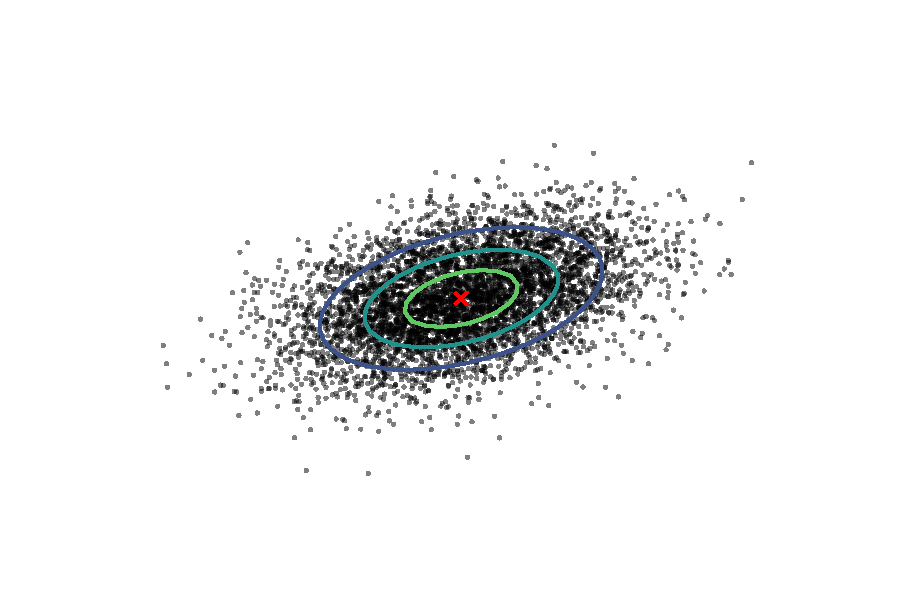
\includegraphics[width=0.8\textwidth]{multivariate_normal.pdf}}
    }

\end{frame}

\begin{frame}{Совместно нормальные величины}
    Вектора $ \mathbf{X} $ и $ \mathbf{Y} $ \textit{совместно} нормально распределены, если вектор $ [\mathbf{X}, \mathbf{Y}] $ нормально распределен.

    \pause
    Pro-tip: не всякая пара нормальных векторов $ \mathbf{X} $ и $ \mathbf{Y} $ совместно нормальна.

    \centerline{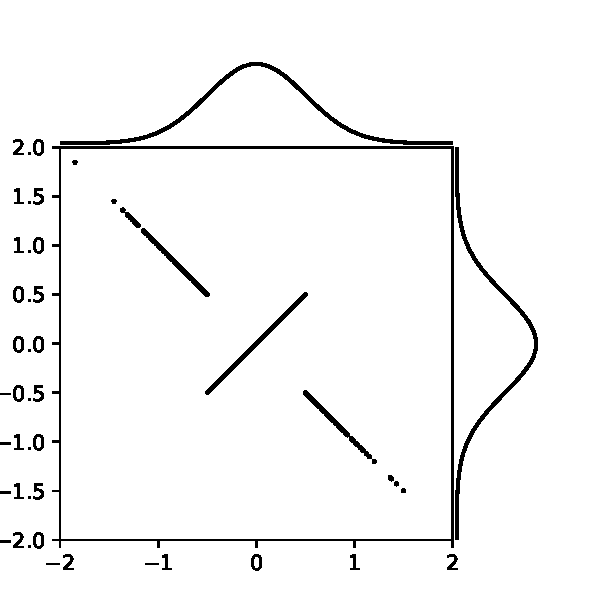
\includegraphics[width=0.5\textwidth]{non-jointly-gaussian.pdf}}
\end{frame}

\begin{frame}{Некоторые полезные свойства}
    «Подвекторы» нормального вектора $ X \sim \mathcal{N}(\mu, \Sigma) $ тоже, конечно, нормальны.

    Если $ X = [X_1, X_2 ] $ и
    $$ \mu = [\mu_1, \mu_2] $$
    $$ \Sigma = \begin{bmatrix} \Sigma_{11} & \Sigma_{12} \\ \Sigma_{21} & \Sigma_{22} \end{bmatrix}, $$

    то

    $$ X_1 \sim \mathcal{N}(\mu_1, \Sigma_{11}), \quad X_2 \sim \mathcal{N}(\mu_2, \Sigma_{22}) $$

    \pause
    В дальнейшем мы будем работать векторами (и процессами) с нулевым матожиданием, поскольку
    $$ X ~ \sim(\mu, \Sigma) \Leftrightarrow X = \mu + Y, \quad Y \sim(0, \Sigma) $$
\end{frame}

\begin{frame}{Обуславливание}
   Пусть $ X, Y $ -- совместно нормальные векторы:

    $$ \begin{bmatrix} X \\ Y \end{bmatrix} \sim \mathcal{N}\left( \begin{bmatrix} 0 \\ 0\end{bmatrix}, \begin{bmatrix} \Sigma_{11} & \Sigma_{12} \\ \Sigma_{21} & \Sigma_{22} \end{bmatrix} \right) $$

    \pause
    \vspace{1cm}
    Тогда \textit{условный} вектор $ X | (Y = y) $ тоже нормален:

    $$ X | (Y = y) \sim \mathcal{N}\left( \Sigma_{12} \Sigma_{22}^{-1} y, \Sigma_{11} - \Sigma_{12} \Sigma_{22}^{-1} \Sigma_{21} \right) $$
\end{frame}


\begin{frame}{Обуславливание с шумом}
    Более естественная постановка: пусть $X, Y$ --- совместно нормальны. Пусть $Y = y + \varepsilon$, где $\varepsilon \sim \mathcal{N}(0, \sigma^2I)$ -- гауссовский шум.

    \pause
    Каково распределение $X | (Y = y + \varepsilon)$?

    $$ \begin{bmatrix} X \\ Y + \varepsilon \end{bmatrix} \sim \mathcal{N}\left( \begin{bmatrix} 0 \\ 0\end{bmatrix}, \begin{bmatrix} \Sigma_{11} & \Sigma_{12} \\ \Sigma_{21} & \Sigma_{22} + \sigma^2I \end{bmatrix} \right) $$

    \pause
    \begin{align*}
    p(X | Y + \varepsilon) &= \frac{p(Y + \varepsilon, X)}{\int p(Y + \varepsilon, X) dX} = \\
    \mathcal{N}\left( \Sigma_{12} (\Sigma_{22}+\sigma^2I)^{-1} Y,\right. & \left. \Sigma_{11} - \Sigma_{12} (\Sigma_{22}+\sigma^2I)^{-1} \Sigma_{21} \right)
    \end{align*}
    \begin{center}
      (считается аналитически)
    \end{center}

\end{frame}

\begin{frame}{Гауссовские процессы}
   \begin{itemize}
    \item<1-> Нормальные случайные вектора -- это обобщение нормальных случайных величин. А что если мы хотим говорить о бесконечномерных обобщениях -- о случайных функциях?

    \item<2-> \textit{Гауссовский процесс} на пространстве $\mathcal{X}$ -- это набор нормальных случайных величин $ \{ f(x) \}_{x \in \mathcal{X}} $, таких что \textit{для любых} $x_1, \ldots, x_N $ конечномерный вектор $[ f(x_1), \ldots, f(x_N) ]$ нормально распределен.

    \item<3-> Обозначение $f(x)$ выбрано не случайно -- можно думать о гауссовском процессе как о \textit{распределении} на функциях в пространстве $\mathcal{X}$.
    \end{itemize}
\end{frame}

\begin{frame}{Гауссовские процессы}
    Гауссовский процесс однозначно задается своим матожиданием и функцией ковариации (также называемой \textit{ядром}).
    \begin{align*} f(x) &\sim \mathcal{GP} (m(x), k(x, x^\prime)) \\
     \mathbb{E}(f(x)) &= m(x) \quad &\forall x \in \mathcal{X} \\
     \text{Cov} ( f(x), f(x^\prime) ) &= k(x, x^\prime) \quad &\forall x, x^\prime \in \mathcal{X} \end{align*}

    \pause
    Для любого $X := [x_1, \ldots, x_N]$ вектор $f_X := [f(x_1), \ldots, f(x_N)]$ гауссовский:

    $$ f_X \sim \mathcal{N}(m_X, K_{XX}), $$
    где
    $$m_X := [m(x_1), \ldots, m(x_N)], \quad K_{XX}[i, j] := k(x_i, x_j)$$
\end{frame}

\begin{frame}{Причем здесь машинное обучение?}
    \begin{itemize}
        \item<1-> Байесовский подход заключается в введении предположений о природе данных и обновлении этих предположений с учетом собственно данных с помощью теоремы Байеса. Мы видели, как такой подход можно применить в параметрических моделях --- предположения строятся относительно параметров модели.

        \item<2-> Гауссовские же процессы позволяют мыслить о данных \textit{непараметрически}. А именно, задавать априорное распределение \textit{функций}, которые порождают наблюдаемые данные, и обновлять это распределение с помощью теоремы Байеса. Это приводит к \textit{Gaussian Process Regression} -- регрессии, основанной на гауссовских процессах.
    \end{itemize}

\end{frame}

\begin{frame}{Gaussian Process Regression}
    \begin{itemize}
      \item Пусть есть некий датасет $(X, Y)$, где $X = [x_1, \ldots, x_N]$, $x_i \in \mathbb{R}^d$, а $Y = [y_1, \ldots, y_N]$, $ y_i \in \mathbb{R}$
      \pause
      \item Данные связаны некоей функциональной зависимостью $y_i = f(x_i)$
          % ,  где $\varepsilon_i \sim \mathcal{N}(0, \sigma^2)$ -- гауссовский шум, независимый с $f$ и $\text{Cov}(\varepsilon_i, \varepsilon_j) = 0$.
      \pause
      \item Функцию $f$ мы не знаем и хотим оценить из данных. Иными словами, каково значение $f(x_*)$ в какой-то произвольной точке $x_*$

    \end{itemize}

\end{frame}

\begin{frame}{Gaussian Process Regression}

    \only<1>{
        Введем априорное предположение, что $f \sim \mathcal{GP}(0, k)$ -- некий гауссовский процесс, и предположим, что мы знаем ковариационную функцию $k$ (позже мы увидим, как оценить $k$ из данных).
    }

    \pause
    Вектор $f(X) = [f(x_1), \ldots, f(x_N)]$ будет нормальным $f(X) \sim \mathcal{N}(0, K_{XX})$ (по определению гауссовского процесса). При этом для произвольного $x_*$ вектор $[f(x_*), f(X)] = [f(x_*), f(x_1), \ldots, f(x_N)]$ тоже будет нормальным (по тому же определению):

    $$ \begin{bmatrix} f(x_*) \\ f(X) \end{bmatrix} \sim \mathcal{N}\left(0,
    \begin{bmatrix} K_{**} & K_{*X} \\ K_{X*} & K_{XX} \end{bmatrix} \right) $$

    \pause
    Кроме того, мы знаем, что $f(X) = Y$. Мы можем посчитать условное распределение:

    $$ f(x_*) | (f(X) = Y) \sim \mathcal{N}\left(K_{*X}K_{XX}^{-1}Y, K_{**} - K_{*X}K_{XX}^{-1}K_{X*} \right) $$

    \pause
    Поскольку эти рассуждения верны для \textit{любого} набора точек $X_* = [x_{*1}, \ldots, x_{*T}]$, мы приходим к \textit{условному} (или \textit{апостериорному}) процессу
    $$ f(x) | (f(X) = Y) \sim \mathcal{GP}\left(k(x, X)K_{XX}^{-1}Y, k(x, X) K_{XX}^{-1} k(X, x) \right) $$

\end{frame}

\begin{frame}{}

    \centerline{\includegraphics<1>[width=\textwidth]{01_gpr_data.pdf}}
    \centerline{\includegraphics<2>[width=\textwidth]{02_gpr_prior.pdf}}
    \centerline{\includegraphics<3>[width=\textwidth]{03_gpr_posterior.pdf}}
    % \centerline{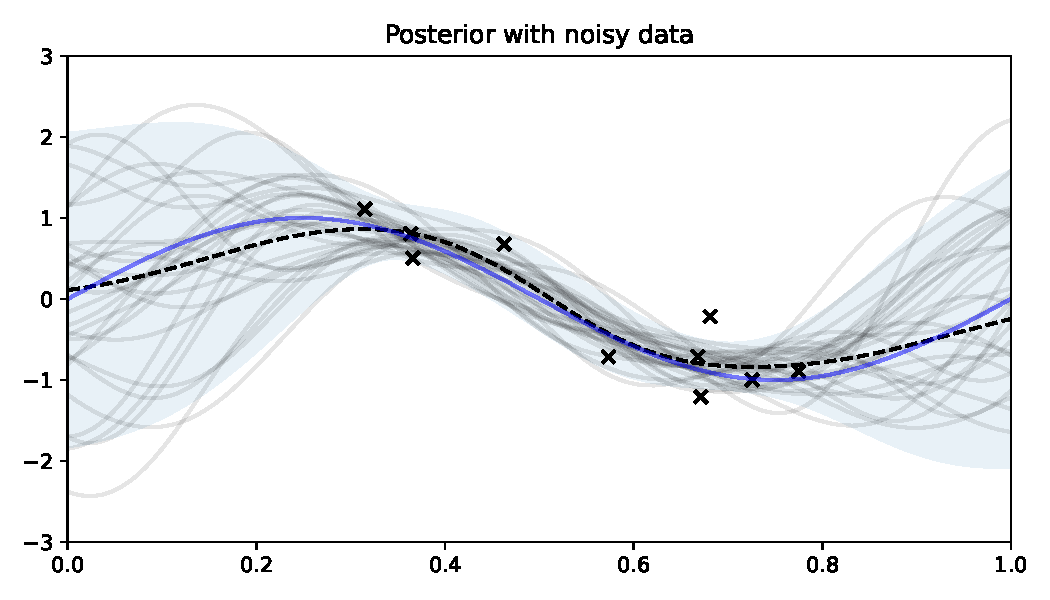
\includegraphics[width=\textwidth]{04_gpr_posterior_noisy.pdf}}

\end{frame}

\begin{frame}{Апостериорный гауссовский процесс}

    \begin{itemize}
        \item<1-> Апостериорный гауссовский процесс предоставляет \textit{распределение} функций, согласованных с данными. % В каждой тестовой точке $x_*$ известен не конкретный ответ модели, а распределение возможных ответов -- в частности, матожидание и дисперсия.

        \item<2-> Дисперсия служит численной мерой неопределенности модели -- чем выше дисперсия, тем более неуверенна модель в своем ответе. % На графиках неопределенность отражают с помощью доверительных интервалов --- например, выше изображен 0.9-доверительный интервал.

    \end{itemize}

\end{frame}

\begin{frame}{Шумные данные}

    Кроме того, обычно предполагают зашумленность данных: $f(X) = Y + \varepsilon$, где $\varepsilon \sim \mathcal{N}(0, \sigma^2 I)$ -- гауссовский шум. В таком случае

    \begin{align*}
      f(x) | (f(X) &= Y + \varepsilon) \sim \mathcal{GP}\Big(k(x, X)(K_{XX} + \sigma^2 I)^{-1}Y, \\
      &k(x, X) (K_{XX} + \sigma^2 I)^{-1} k(X, x) \Big)
    \end{align*}

\end{frame}

\begin{frame}{}

    \centerline{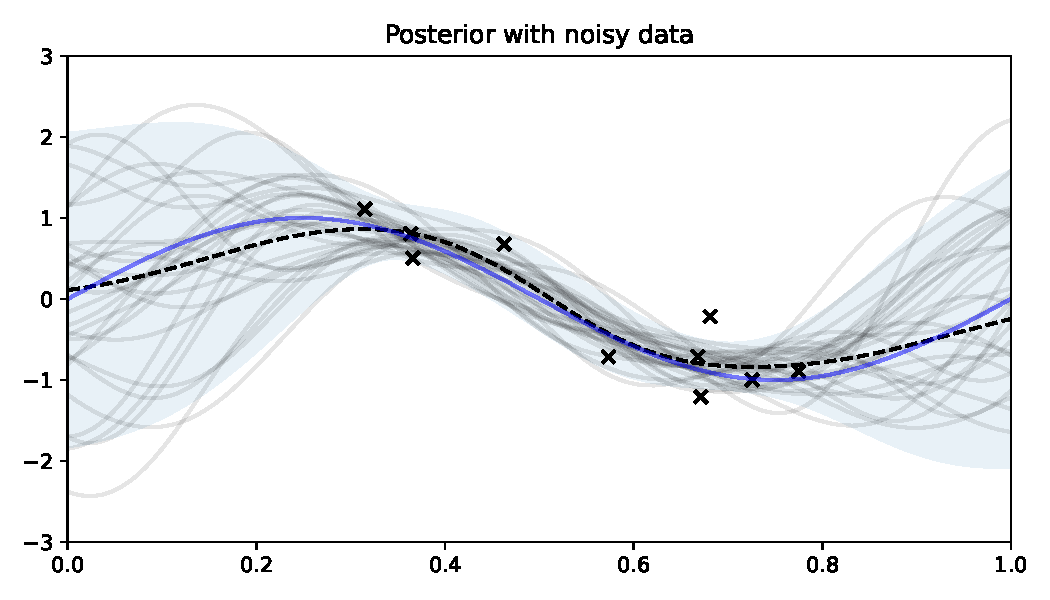
\includegraphics[width=\textwidth]{04_gpr_posterior_noisy.pdf}}

\end{frame}

\begin{frame}{Где Байес?}

    Введем обозначения: $F := f(X)$

    \vfill

    \only<1>{
        априорное распределение (prior):
        $$ p(F) = \mathcal{N}\Big(0, K_{XX} \Big) $$
    }

    \only<2>{
        правдоподобие (likelihood):
        $$ p(Y | F) = \mathcal{N}\Big(F, \sigma^2 I \Big) $$
    }

    \only<3>{
        апостериорное распределение (posterior):
     $$ p (F | Y) = \frac{p(Y | F) p(F) } {\int p(Y | F) p(F) } $$
    }

    \only<4>{
        предсказательное распредение (predictive distribution):
        $$ p(f(x_*) | Y) = \int p(f(x_*) | F) p(F | Y) dF $$
    }

    \only<5>{
        Поскольку все гауссовское, все считается аналитически и:

        \begin{align*} p(f(x_*) | Y) = \mathcal{N}\Big(k(x_*, X)(K_{XX} + \sigma^2 I)^{-1}Y, \\
        k(x_*, X) (K_{XX} + \sigma^2 I)^{-1} k(X, x_*) \Big)
        \end{align*}
    }

\end{frame}

\begin{frame}{«Обучение» гауссовского процесса}

   Для проведения регрессии на основе гауссовских процессов необходимо задать априорный гауссовский процесс, то есть задать его матожидание и функцию ковариации. Как правило, матожидание полагают равным нулю -- всегда можно отнормировать данные. Свойства гауссовского процесса (например, гладкость траекторий) кодируются ядром. Выбор же ядра -- сложный процесс и во многом искусство (хотя и существуют методы автоматического подбора ядра).

\end{frame}

\begin{frame}{Максимизация правдоподобия}

    Как правило, предполагают, что ядро $k$ принадлежит некоторому параметрическому семейству $k = k_\theta, \theta \in \Theta$.

    \pause

    Для подбора оптимальных параметров ядра используется метод максимизации правдоподобия.
    $$L(Y; \theta) = \log p(Y; \theta) = \log \int p(Y | F; \theta) p(F; \theta) dF \longrightarrow \max $$

    \pause
    А именно,

    $$ L(Y; \theta) = -\frac 1 2 Y^\top K_y^{-1} Y - \frac 1 2 \log \det K_Y - \frac n 2 \log 2 \pi \longrightarrow \max$$
    где $K_y = K_{XX} + \sigma^2 I$, а $n$ -- количество данных.

\end{frame}

\begin{frame}{Ядра Матерна}
    Наиболее популярное семейство ядер -- ядра Матерна.

    $$k(x, x^\prime) = k(||x - x^\prime||) = k_\nu(d) = \sigma^2\frac{2^{1-\nu}}{\Gamma(\nu)}\Bigg(\sqrt{2\nu}\frac{d}{\rho}\Bigg)^\nu K_\nu\Bigg(\sqrt{2\nu}\frac{d}{\rho}\Bigg),$$

    где $\Gamma$ -- гамма-функция, $K_\nu$ -- модифицированная функция Бесселя второго рода.

    Параметры ядра:
    \begin{itemize}
        \item<1-> $\sigma^2$ задает дисперсию гауссовского процесса
        \item<2-> $\nu$ отвечает за гладкость траекторий гауссовского процесса
        \item<3-> $\rho$ (параметр масштаба, lengthscale) отвечает за растяжение пространства
    \end{itemize}

\end{frame}

\begin{frame}{Ядра Матерна}

    При $\nu = k + 1/2$, $k = 0, 1, 2, \ldots$ формулы упрощаются и наиболее часто используемые ядра это Матерн-1/2, Матерн-3/2, Матерн-5/2.

    При $\nu \to \infty$ ядро Матерна совпадает с другим известным ядром -- гауссовским:
    $$k(x, x^\prime) = \sigma^2 \exp\left(-\frac{||x - x^\prime||^2}{2 \rho^2}\right)$$

\end{frame}

\begin{frame}{Другие ядра}
    Рассматривают и другие семейства ядер, такие как Rational Quadratic, Piecewise Polynomial, Standard Periodic, и т.д.

    В целом любая положительно-определенная функция может быть ядром.

    \pause
    Кроме того, если $k_1(x, x^\prime), k_2(x, x^\prime)$ -- ядра, то $k_1(x, x^\prime) + k_2(x, x^\prime)$, $k_1(x, x^\prime) k_2(x, x^\prime)$ -- ядра.

    Если $k_1(x, x^\prime)$, $k_2(y, y^\prime)$ -- ядра, то $k(z, z^\prime) = k_1(x, x^\prime) + k(y, y^\prime)$, $k(z, z^\prime) = k(x, x^\prime) k(y, y^\prime)$ -- ядра, где $z = [x, y]$.
\end{frame}

\begin{frame}{Формула Матерона}
    Апостериорный процесс $f | Y$ задается аналитическими матожиданием и ковариационной функцией. % Поэтому, казалось бы, легко получать сэмплы (траектории) этого процесса в произвольных точках $X_* := [x_{*1}, \ldots x_{*T}]$:

    \begin{align*} f(X_*) \sim \mathcal{N}\Big(\mu := k(x_*, X)(K_{XX} + \sigma^2 I)^{-1}Y, \\ \Sigma := k(x_*, X) (K_{XX} + \sigma^2 I)^{-1} k(X, x_*) \Big) \end{align*}

    \pause
    $$ f(X_*) = \mu + \Sigma^{1/2} u, \quad u \sim \mathcal{N}(0, I) $$

    Это требует вычисления корня из матрицы $\Sigma$ размера $(T, T)$ (сложность $O(T^3)$ операций). Если $T$ велико, то это фактически невозможно.
\end{frame}

\begin{frame}{Формула Матерона}
    Альтернативный способ предоставляет формула Матерона.

    $$ f(x_*) | Y = f(x_*) + (K_{XX} + \sigma^2 I)^{-1}(Y - \varepsilon) $$

    Пусть мы умеем каким-то образом эффективно получать траектории априорного процесса $f$ как функции от $x$. Тогда
    можно автоматически получать траектории процесcа $f | Y$ как функции от $x_*$, \textit{корректируя} априорные сэмплы поправкой, вносимой наблюдаемыми данными.
\end{frame}

% \begin{frame}{}

% \centerline{\includegraphics[width=\textwidth]{matheron_overview-1.pdf}}

% \end{frame}

\begin{frame}{Зачем}

\begin{itemize}
    \item Байесовский подход, в котором всё можно посчитать \only<2->{\tiny(почти).} \normalsize
    \item<3-> Оценка неопределенности.
    \item<4-> Small data.
    \item<5-> Ядра существуют для необычных пространств --- графы, римановы многообразия и т.п.
\end{itemize}
    % Регрессия на основе ГП важна в случаях, когда важна оценка неопределенности модели. В частности, например, в проблемах small data, байесовской оптимизации и т.п.

    % \pause
    % Кроме того, ГП определяется своим ядром, и существуют естественные обобщения ядер на неевклидовы пространства --- например,  Тем самым, можно рассматривать регрессию на данных, которые "живут" в странных пространствах.
\end{frame}

\begin{frame}{Проблемы ГП-регрессии}

\begin{itemize}
    \item<1-> \textbf{Big data}. Поскольку «обучение» ГП требует обращения матрицы $K_{XX}$, размер которой зависит от количества данных, использование ГП-регрессии на больших данных затруднено. Обращение большой плотной плохо обусловленной матрицы на каждой итерации градиентного спуска -- вычислительно тяжелая задача. Существует методы \textit{sparse Gaussian processes}, которые в определенной степени решают эту проблему.
    \item<2-> \textbf{Large dimensions}. ГП-регрессия плохо работает на данных в пространствах большой размерности (например, картинки). Существуют подходы для работы с такими данными.
\end{itemize}

\end{frame}

\begin{frame}{Это еще не всё}

GP in Machine Learning --- активно развивающаяся область науки.

Стандартная книжка по гауссовским процессам в машинном обучении -- \href{http://www.gaussianprocess.org/gpml/chapters/RW.pdf}{Gaussian Processes for Machine Learning} (доступна онлайн).

\end{frame}

\begin{frame}{}

    \centerline{Спасибо!}

\end{frame}

\end{document}
